\section{UML (Unified Modeling Language)}

\begin{comment}

De oorspronkelijke bedoeling bij het creëren van UML was om de grootste gemene deler te vinden bij de verschillende bestaande technieken en zo de beste methode te bekomen, maar dit bleek niet eenvoudig (denk maar aan de methodestrijd die heel hevig gewoed heeft) en uiteindelijk is het het kleinste gemeen veelvoud geworden: alle bestaande methodes en technieken zijn erin terug te vinden. De kunst bestaat er dus in die dingen te gebruiken die op dat moment nodig zijn. Vandaar ook dat UML geen methodologie genoemd kan worden, maar een taal, een notatiewijze geworden is...

Hierbij mag het werk van OMG (Object Management Group), de leidende organisatie voor standaarden in het domein van object oriëntatie, niet onderschat worden. De RTF (Revision task Force) doen al het voorbereidend werk naar volgende versies toe.

%afbeelding nog plaatsen

\begin{center}
\includegraphics[width=4in]{img/}%
\captionof{figure}{text}
\label{labelname}%
\end{center}

UML invloeden: naast de invloeden van de stichters, zijn er vanuit andere methoden ook invloeden geweest: Bertrand Meyer heeft het contractsgewijs werken geïntroduceerd dankzij het werken met pre- en postcondities, Harel heeft de toestandsdiagrammen toegevoegd, de groep rond Gamma heeft het werken met patronen een plaats gegeven in de taal, Hewlet-Packard heeft de collaboratiediagrammen toegevoegd.

\end{comment}

De diagrammen zijn de eigenlijke afbeeldingen van de modelelementen die het systeem voorstellen. Verder in de cursus wordt uitgebreid tijd besteed aan elk van de diagrammen.

\subsection{Overzicht van de diagrammen}

Gezien de vele invloeden waar UML aan onderhevig was, zijn er ook een heleboel diagrammen die op verschillende momenten in de systeemontwikkeling gemaakt kunnen worden. Hieronder volgt een beknopte beschrijving waar een aantal van de meest gebruikte diagrammen beschreven worden. Verder in dit hoofdstuk worden deze nog meer gedetailleerd uitgewerkt en wordt ook aangeduid welk diagram in welke ontwikkelingsfase uitgewerkt kan worden.

\subsubsection{Klassendiagram}

In een klassendiagram worden de klassen getoond, waarbij men in de klassen weergeeft welke dingen belangrijk zijn in het systeem, welke kenmerken deze dingen hebben (d.m.v. de attributen) en hoe deze dingen zich gedragen (d.m.v. de operaties). Verder vindt men in het klassendiagram de manier waarop de klassen onderling samenhangen.

\subsubsection{Objectdiagram}

Een objectdiagram is een instantiatie van een klassendiagram. Hierin wordt een concreet voorbeeld van een klassendiagram uitgewerkt.

\subsubsection{Use-case diagram : MOGELIJKE EXAMENVRAAG}

Een use-case is een beschrijving van het gedrag van een systeem vanuit het standpunt van de gebruiker. In het use-case diagram worden de functionaliteiten van het systeem getoond en daarenboven wie of wat betrokken zal zijn bij deze functionaliteiten. \textcolor{red}{Een use-case beschrijving wordt een blackbox beschrijving genoemd, aangezien enkel beschreven wordt wat er gebeurt vanuit het zichtpunt van de gebruiker en niet hoe dat gebeurt.}
\newpage
\subsubsection{Toestandsdiagram}

Elk object bevindt zich op een bepaald moment in een bepaalde toestand. In het toestandsdiagram worden de verschillende mogelijke toestanden van de objecten gevisualiseerd, alsook de manieren waarop een object kan overgaan van één toestand naar een andere toestand.

\subsubsection{Activiteitendiagram}

De activiteiten die binnen een use-case of binnen het gedrag van een object na elkaar plaatsvinden, vind je in een activiteitendiagram. Een activiteitendiagram wordt typisch gebruikt om een werkstroom voor te stellen (workflow diagram).

\subsubsection{Sequentiediagram}

In een sequentiediagram wordt de interactie weergegeven die plaats vindt tussen de verschillende objecten in de uitvoering van een use-case. Hierbij worden de interacties gezien in functie van de tijd.

\subsubsection{Collaboratiediagram}

In een collaboratiediagram wordt de interactie die plaats vindt tussen de verschillende objecten in een use-case voorgesteld. Hierbij worden de interacties niet meer gezien in functie van de tijd, maar de samenwerking.
De verschillende elementen (objecten) van een systeem werken samen om de doelstellingen van het systeem te verwezenlijken.

\subsubsection{Componentendiagram}

In een componentendiagram vind je die verschillende componenten van het systeem, hierbij moet je een component zien als een fysisch deel van een systeem dat deel uitmaakt van de software-implementatie van het systeem.

\subsubsection{Deployment diagram}

Het deployment diagram toont de fysische architectuur van een computersysteem, het kan de componenten en de randapparaten beschrijven, de verbindingen ertussen laten zien en aangeven welke software op de verschillende machines aanwezig is.
\newpage
\subsection{Statische en dynamische diagrammen}

de statische diagrammen geven een statisch beeld van het systeem. Dat betekent dat ze stabiel blijven, ongeacht het moment waarop ze bekeken worden. Een voorbeeld is het klassendiagram: dit geeft een statisch beeld op de objecten en hun onderlinge relaties. Ongeacht op welk moment het systeem via dit diagram bekeken wordt, zullen deze relaties altijd hetzelfde zijn.

De dynamische diagrammen, daarentegen, kunnen een ander beeld geven van het systeem als ze op een ander moment bestudeerd worden. Een voorbeeld is het toestandsdiagram: al naargelang het moment waarop dit bekeken wordt, kan het object zich in een andere toestand bevinden.

\begin{center}
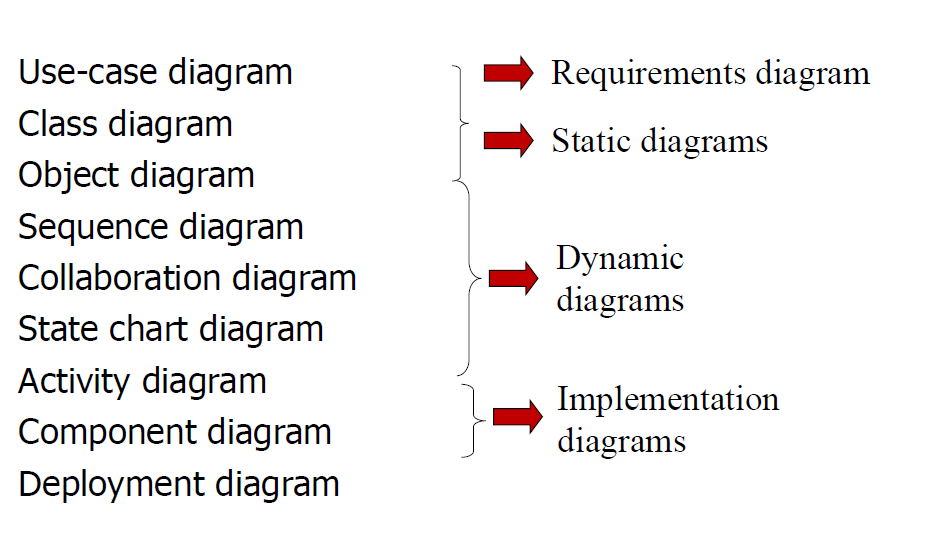
\includegraphics[width=4in]{img/overviewumllen}%
\end{center}

